\documentclass[12pt,a4paper,aspectratio=169]{beamer}
\usepackage[utf8]{inputenc}
\usepackage[T1]{fontenc}
\usepackage{amsmath}
\usepackage{minted}
\usepackage{amssymb}
\usepackage{graphicx}
\begin{document}
	\author{Programação C e 8051}
	\title{"Aula" exercícios/dúvidas/revisão}
	%\subtitle{}
	%\logo{}
	\institute{Universidade Federal de Santa Catarina}
	\date{23/10/2020}
	%\setbeamercovered{transparent}
	\setbeamertemplate{navigation symbols}{}
		
	\begin{frame}[plain]
		\maketitle
	\end{frame}

\begin{frame}
	Ideia geral dessa reunião:
	
	\begin{itemize}
		\item Aula totalmente não oficial. Pensem como uma ajudinha a mais de alguém que já fez a matéria, e não de alguém que é expert no campo (como os professores).
		\visible<2->{\item Colaborativo! Eu pergunto coisas pra vocês, vocês perguntam coisas pra mim. Se eu não souber a resposta, buscamos juntos.}
		\visible<3->{\item \textbf{Todo} o material, incluindo códigos, slides, a gravação da aula e qualquer outra coisa ficará disponível pra vocês a partir fim da aula.}
		\visible<4->{\item Adendo: pra que ninguém fique desconfortável em fazer perguntas e interagir, se assume que a gravação da aula vai ficar apenas entre os colegas, okay?}
	\end{itemize}
\end{frame}

\begin{frame}
	Programação de hoje:
	\begin{itemize}
		\visible<2->{\item Princípios de verificação de código.}
		\visible<3->{\item Discussão sobre tratadores de interrupção e resolução de um problema pequeno.}
		\visible<4->{\item Revisão sobre \texttt{SFR}s.}
		\visible<5->{\item Tática de resolução de problemas e como resolução de um problema que vocês já fizeram.}
		\visible<6->{\item Resolução de um problema de prova, começo ao fim.}
	\end{itemize}
\end{frame}

\begin{frame}
	\begin{itemize}
		\item Composição de procedimentos: Uma coisa por vez.
		
		\visible<2->{\item Escreve o código $\rightarrow$ Verifica o funcionamento $\rightarrow$ Usa esse código num sistema.}
		
		\visible<3->{\item Exemplo de um dos exercícios (faremos depois):}

	\end{itemize}
	\visible<3->{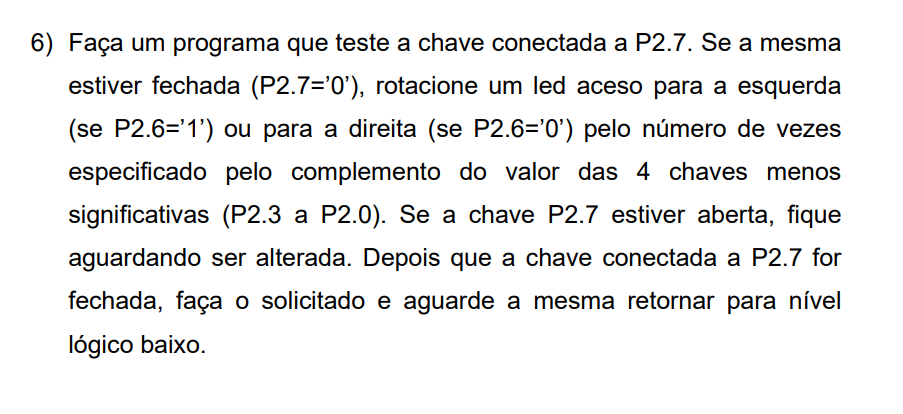
\includegraphics[scale = 0.4]{imagens/exemplo6_clean.PNG}}

	\begin{itemize}
			\visible<4->{\item Parte fundamental: rotacionar LED. Resto: Firula.}
	\end{itemize}
\end{frame}

\begin{frame}[fragile]
	\begin{itemize}
			\item \textit{temperatura} deveria receber \texttt{P2}, mas recebe \texttt{P1}:
	\end{itemize}

	\begin{minted}{C}
	
	void main(void){
		if(verificar_temperatura()){
			acender_aquecedor(); //não funciona!
		}
	}
	void verificar_temperatura(){
		temperatura = P1; //mas devia ser P2...
	}
	\end{minted}
	\begin{itemize}
		\item Se você não verificou o funcionamento de \texttt{verificar\_temperatura()} (e tinha um erro) e escreveu \texttt{acender\_aquecedor()}, se dobra o número de funções a procurar o possível erro! Pode ficar \textbf{MUITO} difícil de debuggar.
	\end{itemize}
\end{frame}

\begin{frame}[fragile]
	Façam seus tratadores de interrupção curtos e grossos.
	\visible<2->{Estudo de caso de um código que vocês escreveram (o código nunca vai pra frente):}
	
	\begin{minted}{C}
			
void c51_int0 (void)  interrupt 0 {
	rotesq();     
}
		
void rotesq (){
	while(1){
		if(leds == 0xFE) leds = 0x7F;
		else leds = (leds >> 1) | 0x80;
		
		P1 = leds;
		delay();
	}
}

	\end{minted}
\end{frame}

\begin{frame}
	\begin{itemize}
		\item \visible<1->{Qual o principal problema no nesse código e como possivelmente eu ia saber que esse era o problema?}
		
		\item \visible<2->{Chamadas de função fazem uso de \texttt{pop} e \texttt{push}, ou seja: mexem com o stack toda vez que se chama a função.}
	
		\item \visible<3->{Se você nunca retornar da função e fazer contínuas chamadas $\rightarrow$ stack overflow (chamadas recursivas teriam o mesmo efeito).}
		
		\item \visible<4->{Como eu \textbf{possivelmente} poderia saber disso?}
	
	\end{itemize}	

	
\end{frame}

\begin{frame}
	Do manual do 8051:
	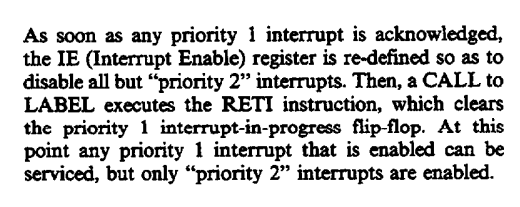
\includegraphics[scale = 0.8]{imagens/EAinterrupt.PNG}
\end{frame}

\begin{frame}[fragile]
	\begin{itemize}
		\item Alternativa de código (extremamente parecida com os exemplos da aula!):
	\end{itemize}
	\begin{minted}{C}
	bit state = 0;
	void main(void) {
		while(state)
		{
			rotesq();
		}
	}
	
	void c51_int0 (void) interrupt 0 {
	state = 1;
	}
	
	\end{minted}
\end{frame}

\begin{frame}[fragile]
	\texttt{SFR} - Special Function Register
	\begin{minted}{C}
		sfr name = address;
		//em reg51.h
		sfr P0   = 0x80;
		sfr P1   = 0x90;
		sfr P2   = 0xA0;
		sfr P3   = 0xB0;
	\end{minted}
\end{frame}

\begin{frame}[fragile]
	\texttt{sbit} e bit-addressable SFRs
	\begin{minted}{C}
	sbit name = sfr-name ^ bit-position; //caso 1
	sbit name = sfr-address ^ bit-position; //caso 2
	sbit name = sbit-address; //caso 3
	\end{minted}
\end{frame}

\begin{frame}[fragile]
	Caso 1:
	
	\begin{minted}{C}
	sbit name = sfr-name ^ bit-position;
	
	/*Onde sfr-name deve ser divisível por 8 
	(Qual a razão?)*/
	sfr P0   = 0x80;
	sfr P1   = 0x90;
	
	sbit P0_0 = P0^0;
	sbit P0_1 = P0^1;
	sbit batata = P1^4;
	P0_0 = 1;

	\end{minted}
	
	\begin{itemize}
		\item Pois a memória é dividida em bytes! Ou 8 bits.
	\end{itemize}
\end{frame}

\begin{frame}[fragile]
	Caso 2:
	
	\begin{minted}{C}
	sbit name = sfr-address ^ bit-position;
	
	/*Onde sfr-address deve ser divisível por 8 
	(Qual a razão?)*/
	sfr P0   = 0x80;
	sfr P1   = 0x90;
	
	sbit P0_0 = 0x80^0;
	sbit P0_1 = 0x90^1;
	sbit batata = 0x90^4;
	
	\end{minted}
	
	\begin{itemize}
		\item Pois a memória é dividida em bytes! Ou 8 bits.
	\end{itemize}
\end{frame}

\begin{frame}
	\begin{itemize}
		\item Nota: Nem todo SFR é bit-addressable. Só aqueles que terminam em 0 ou 8.\\
		
		\item Curiosidade: No entanto, o C51 tem um hack pra isso. Procurem a documentação.\\
		
		\visible<2->{\item Quem vocês xingam sobre isso: Projetistas de silício da Intel.}
	\end{itemize}
\end{frame}

\begin{frame}[fragile]
	Caso 3:
	
	\begin{minted}{C}
	sbit name = sbit-address;
	
	 /* Onde sbit-address deve estar entre 0x80-0xFF.
	 (Qual a razão?) */
	sfr P0   = 0x80;
	sfr P1   = 0x90;
	
	sbit P0_0 = 0x80;
	sbit P0_1 = 0x81;
	sbit batata = 0x93; //P1^4
	
	\end{minted}
\end{frame}

\begin{frame}
	\begin{itemize}
		\item Exemplo no Keil, do arquivo \texttt{reg51.h}.
	\end{itemize}
\end{frame}

\begin{frame}
	Exercícios!!!
	
	\begin{itemize}
		\item Uma prova antiga.
		\item Exercício 6 do lab 2. (rotacionar LEDs)
	\end{itemize}
\end{frame}

\begin{frame}
	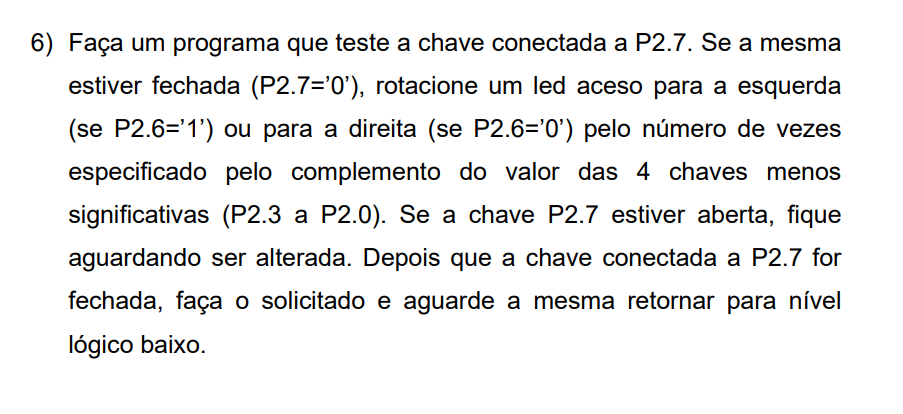
\includegraphics[scale = 0.6]{imagens/exemplo6_clean.PNG}
\end{frame}

\begin{frame}
	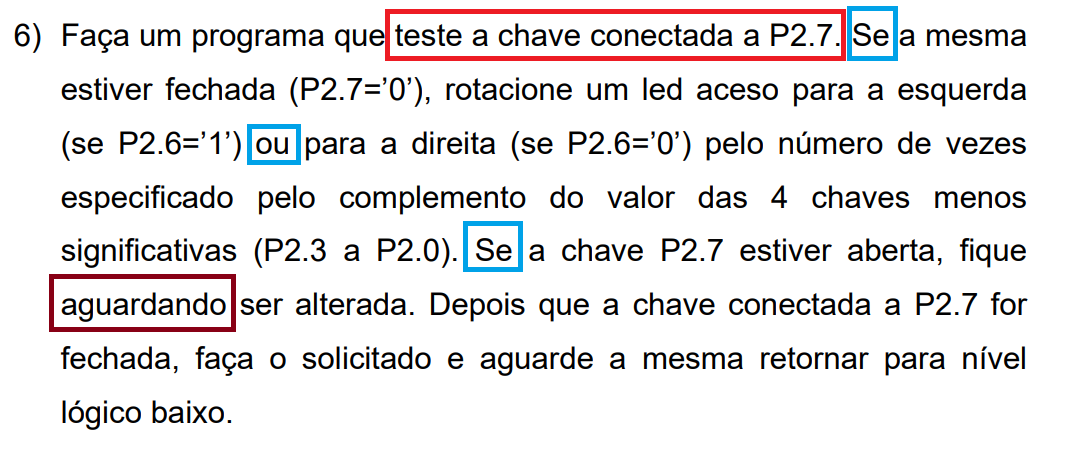
\includegraphics[scale = 0.5]{imagens/exemplo6.PNG}
\end{frame}

\begin{frame}
	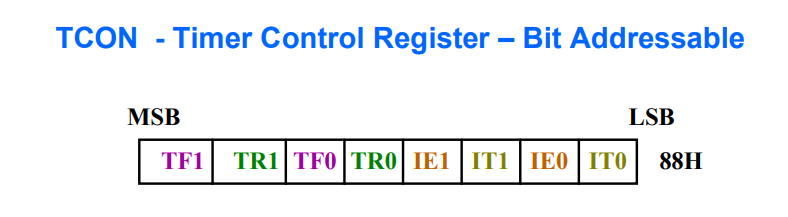
\includegraphics[scale = 0.5]{imagens/TCON.PNG}
\end{frame}

\begin{frame}
	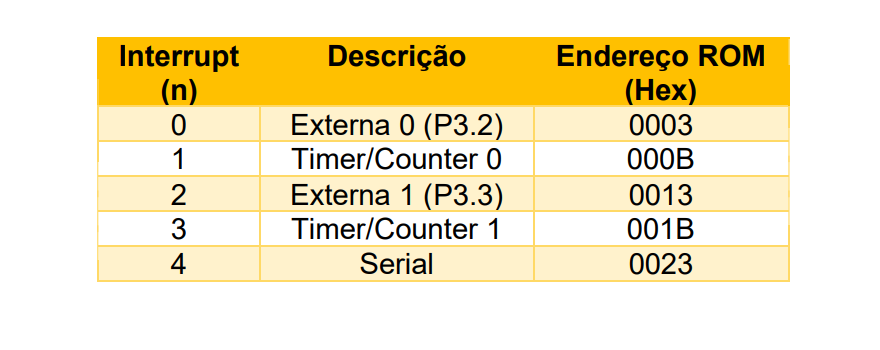
\includegraphics[scale = 0.5]{imagens/interrupts.PNG}
\end{frame}

\begin{frame}
	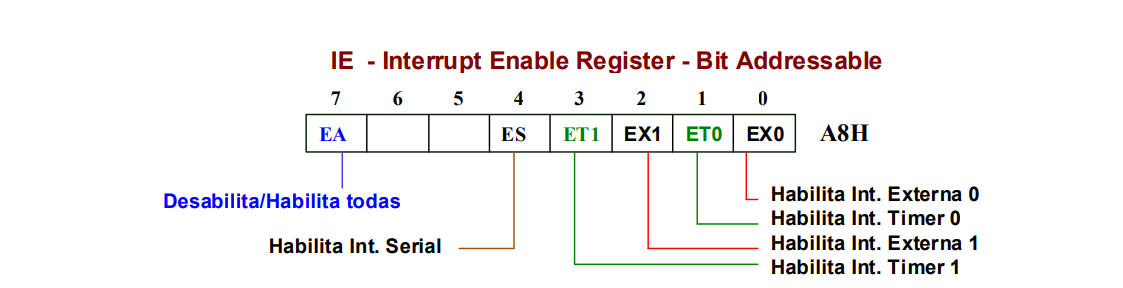
\includegraphics[scale = 0.5]{imagens/IE.PNG}
\end{frame}

\end{document}